\documentclass[dvipsnames]{beamer}

\usetheme{Madrid}
\usecolortheme[named=SeaGreen]{structure}

\usepackage[utf8]{inputenc}
\usepackage[spanish]{babel}
\usepackage{marvosym}
\usepackage{graphicx}

%----------------------------------------------------------------------------------------
%	TITLE PAGE
%----------------------------------------------------------------------------------------

\title[Progress on Muon Telescope]{Muon Telescope} % The short title appears at the bottom of every slide, the full title is only on the title page

\author{Cristóbal Morales} % Your name
\institute[PUC] % Your institution as it will appear on the bottom of every slide, may be shorthand to save space

{
\textit{cimorales2\MVAt uc.cl}\\ % Your email address
Pontificia Universidad Católica de Chile\\ % Your institution for the title page
}
\date{20 October 2017} % Date, can be changed to a custom date

\begin{document}

\begin{frame}
\titlepage %Print the title page as the first slide
\end{frame}

%------------------------------------------------

\begin{frame}{Angle Distribution}
    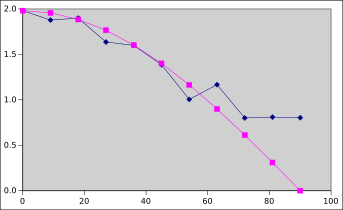
\includegraphics[scale=0.5]{angle_dis.svg}
\end{frame}

%------------------------------------------------


\end{document}
